% mn2esample.tex
%
% v2.1 released 22nd May 2002 (G. Hutton)
%
% The mnsample.tex file has been amended to highlight
% the proper use of LaTeX2e code with the class file
% and using natbib cross-referencing. These changes
% do not reflect the original paper by A. V. Raveendran.
%
% Previous versions of this sample document were
% compatible with the LaTeX 2.09 style file mn.sty
% v1.2 released 5th September 1994 (M. Reed)
% v1.1 released 18th July 1994
% v1.0 released 28th January 1994

\documentclass[usenatbib]{mn2e}
\let\bibhang\relax
\usepackage{graphicx,subfigure}
\usepackage{bm}
\usepackage{longtable}
\usepackage{float}
\usepackage{amsmath,amssymb,graphicx}
\usepackage{rotating}
\usepackage{color}
\usepackage{cite}
\usepackage{epstopdf}

\bibliographystyle{mn2e}
\bibdata{sources}

% If your system does not have the AMS fonts version 2.0 installed, then
% remove the useAMS option.
%
% useAMS allows you to obtain upright Greek characters.
% e.g. \umu, \upi etc.  See the section on "Upright Greek characters" in
% this guide for further information.
%
% If you are using AMS 2.0 fonts, bold math letters/symbols are available
% at a larger range of sizes for NFSS release 1 and 2 (using \boldmath or
% preferably \bmath).
%
% The usenatbib command allows the use of Patrick Daly's natbib.sty for
% cross-referencing.
%
% If you wish to typeset the paper in Times font (if you do not have the
% PostScript Type 1 Computer Modern fonts you will need to do this to get
% smoother fonts in a PDF file) then uncomment the next line
% \usepackage{Times}

%%%%% AUTHORS - PLACE YOUR OWN MACROS HERE %%%%%

\newcommand{\f}[2]{\frac{#1}{#2}}

% denotes an edit in the actual body of the text.
%% denotes a personal comment by the editor.

%%%%%%%%%%%%%%%%%%%%%%%%%%%%%%%%%%%%%%%%%%%%%%%%


\title[]{High Altitude Ballooning: A Comprehensive Review}
\author[Amanda Maxham, etc.]{Amanda Maxham\thanks{E-mail:
maxham@physics.unlv.edu (AM); lujane@unlv.nevada.edu (EL); leeh44@unlv.nevada.edu (JL)} Jake Lee, and Eric Lujan\\
Department of Physics and Astronomy, University of Nevada, Las Vegas, Las Vegas, NV, 89124, U.S.A.}
\begin{document}

\date{Accepted . Received ; }

\pagerange{\pageref{firstpage}--\pageref{lastpage}} \pubyear{2013}

\maketitle

\label{firstpage}
\begin{abstract}
This will be re-written after the paper is completed
\end{abstract}
\section{Introduction}
With the recent interest in high altitude ballooning from universities, companies, and amateur scientists, many are seeking for more information on the science behind high altitude ballooning. This paper reviews some of the science, equipment and calculations behind  a successful launch and features a few interesting student projects.
%%The introduction should include the motive and purpose of the paper. The reader should be able to recognize the purpose of the entire paper by just reading this paragraph.

\section{Balloon Lift}

\subsection{Net Lift}

Two major forces act on a free-floating balloon along the z-axis. The positive buoyant force, $F_B$, and the gravitational force, $F_g$. These forces can be combined to find the net lift force of the balloon:

\begin{equation} 
\Sigma F= F_B - F_g
\end{equation}

The buoyant force, $F_B$, can be calculated by using the Archimedes Equation:

\begin{equation} \label{eq:Buoyancy}
F_{B} = \rho_f V g
\end{equation}

where $\rho_f$ is the density of the displaced fluid in $kg/m^3$ (in our case, air), V is the volume of the balloon in $m^3$, and g is the acceleration due to gravity in $m/s^2$. Kilograms is used for $F_{B}$ instead of newtons , as it is more convenient for our application.

The density and pressure of the atmosphere changes with altitude, causing the buoyant force to change throughout the flight. The data for density and pressure is available in the 1976 US Standard Atmosphere for up to 86 kilometers. The volume of the gas at in the balloon at STP can be measured with a flowmeter attached to the gas source. Additional factors effect the buoyant force, and will be covered in section 1.2.

The gravitational force, $F_g$, is the mass of the entire balloon, including the payloads, the balloon itself, and the gas inside the balloon:

\begin{equation}
F_{g}=m_b-m_p-(\f{n*M}{1000})
\end{equation}

where $m_b$ is the mass of the balloon, $m_p$ is the mass of the payload, $n$ is the moles of gas in the balloon, and $M$ is the mass of the gas in grams.

When both of these forces are combined into equation 1, we end up with the net lift, or $\Sigma F$.

\subsection{Change In Lift With Altitude}
\label{sec:backpressure}

During several experimental deployments, it was observed that the latex balloon was able to reach a state of neutral buoyancy without any manual modifications to the balloon during its flight. This suggests that the lift force of the balloon changes throughout the flight with altitude. Of the two forces that influence $\Sigma F$, only $F_B$ can potentially change, as the mass of the balloon should stay the same throughout the flight (unless the mass is modified intentionally).

Two factors are involved with buoyancy: The volume of the gas and the density of the air. The density of the air changes throughout the flight due to change in altitude. The volume of the gas also changes throughout the flight, and can be modeled with the gas-specific ideal gas law. 

\begin{equation}
P_{gas} = \frac{R_{specific}T}{v}
\end{equation}
Where $P_{gas}$ is the pressure of the gas in pascals, $v$ is the volume in $m^3$, $R_{specific}$ is defined as $\frac{R}{M}$, where $R$ is the universal gas constant and $M$ is the molar mass of the gas in $g$, and $T$ is the temperature of the gas in Kelvin. We assume that the temperature inside the balloon is equal to the temperature of the atmosphere, the data for which can be found in the 1976 US Standard Atmosphere.
However, assuming that the pressure inside the balloon equals the pressure outside the balloon (the balloon expands to match the pressure), the volume of the balloon changes proportionally to the density of the atmosphere, resulting in no change in lift. This is contradictory to our observations; therefore, there has to be another factor that effects the volume. This is the back pressure of the elastic latex. 

Various models exist for sphere rubber shells (also known as rubber balloons), including the Gent model and the Mooney-Rivlin model. This paper will be focusing on the Mooney-Rivlin model to keep the paper concise.

The modified Mooney-Rivlin model for the back pressure of an incompressible spherical rubber shell is as such:

\begin{equation}
P_{back} = 2\mu\frac{t_0}{r_0}((\frac{t_0}{r_0})-(\frac{t_0}{r_0})^7)(1+\frac{1-\alpha}{\alpha}(\frac{t_0}{r_0})^2)
\end{equation}

Where $\mu$ is the shear modulus in $Pa$, $\alpha$ is a constant, $r_0$ is the unstretched radius of the balloon in $m$, and $t_0$ is the thickness of the balloon in $m$. Setting $\alpha$ as 1 results in the neo-Hookean model. While this is useful for small stretches, it does not accurately describe experimental data at high values of strain "Kanner". Müller suggests values of $\f{10}{11}$ for $\alpha$ and $300 kPa$ for $\mu$ to accurately model the radius of the rubber balloon. 
Note that for applicative purposes, it is possible to calculate $r_0$ by measuring the volume of gas at STP with a flowmeter and assuming that the balloon is a sphere. More specifically,

\begin{equation}
	r_0 = ((3*v)/(4*pi))^\frac{1}{3}
\end{equation}

Additionally, $t_0$ can be calculated through $r_0$.
\begin{equation}
	t_0 = \frac{mb}{4*pi*r_0^2*\rho_r}
\end{equation}
Where $\rho_r$ is the density of the rubber. " " suggests a value of 1100 $kgm^-3$

Including the back pressure of the balloon, the internal pressure of the balloon can now be expressed as such.

\begin{equation}
P_B = P_{gas} - P_{back}
\end{equation}
\begin{equation}
P_B = \f{R_{specific}T}{v} - 2\mu\frac{t_0}{r_0}((\frac{t_0}{r_0})-(\frac{t_0}{r_0})^7)(1+\frac{1-\alpha}{\alpha}(\frac{t_0}{r_0})^2)
\end{equation}

Since we are assuming that the atmospheric pressure and the pressure inside the balloon are equal, we result in this equation.

\begin{equation}
P_A = P_B
\end{equation}
\begin{equation}
P_A - \f{R_{specific}T}{\f{4}{3} \pi r^3} + 2\mu\frac{t_0}{r_0}((\frac{t_0}{r_0})-(\frac{t_0}{r_0})^7)(1+\frac{1-\alpha}{\alpha}(\frac{t_0}{r_0})^2) = 0
\end{equation}

Where $P_A$ is the atmospheric pressure. By applying the correct values for specific altitudes, the equation can be solved $r$, which can be used to solve for the volume of the balloon, which in turn can be used to calculate the buoyant force of the balloon for alitutde intervals using Equation \ref{eq:Buoyancy}.

\begin{figure}
\begin{center}
  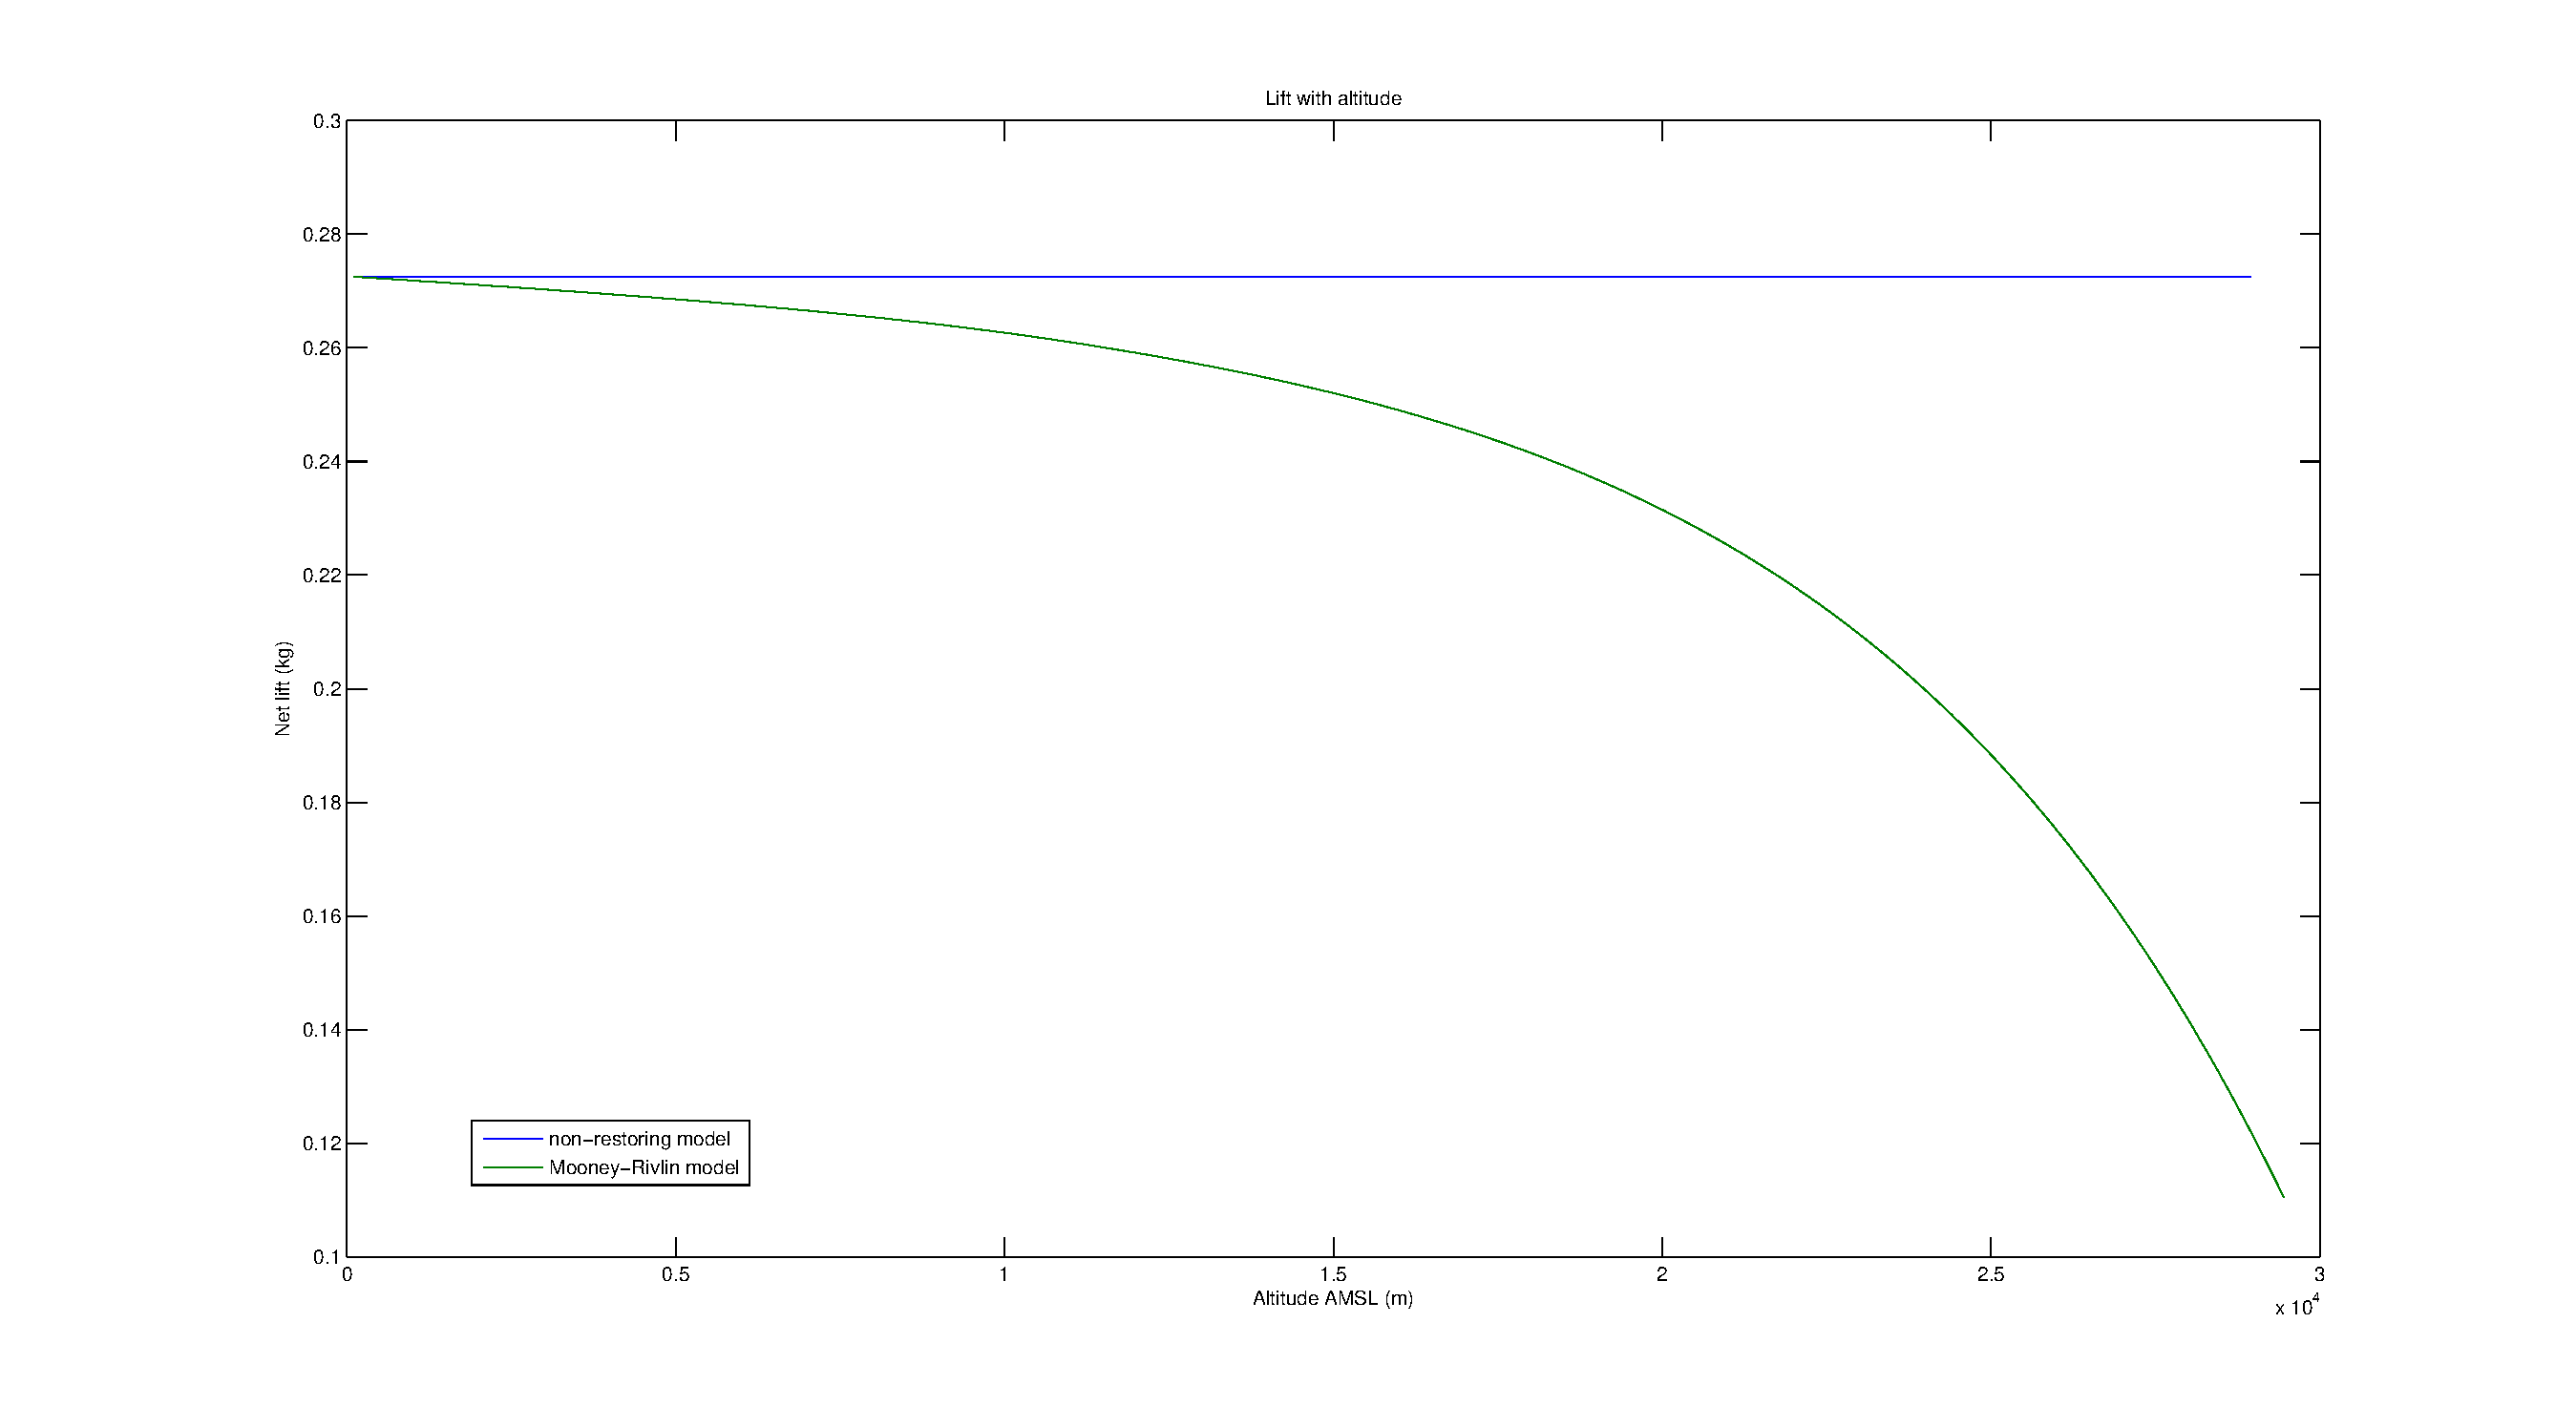
\includegraphics[width=0.5\textwidth]{lift.eps}
  \caption{A lift vs. altitude plot. The following values were used: $m_b = 1.616$, $m_p = 0.189$, $M = 2.0158$, and $v_{stp} = 1.8334$ (which is used to calculate $r_0$)}
\end{center}
\end{figure}

\subsection{Neutral Buoyancy}

Achieving neutral buoyancy is the foundation of achieving long-distance balloon flight. When a balloon is neutrally buoyant, it is able maintain a constant altitude and stay within fast-moving air currents without bursting. Most trans-continental and trans-oceanic high-altitude balloon flights attain near-neutral buoyancy in order to achieve the longest float time possible.

Neutral buoyancy is achieved when the forces on the balloon along the z-axis reach a point of equilibrium such that:

\begin{equation}
\Sigma F = 0 = F_B - F_g
\end{equation}

which can be manipulated to show the relation between buoyant force and gravity:

\begin{equation} \label{eq:NBEQ}
	F_B = F_g
\end{equation}

In practice, this is acheived by filling the balloon with a specific volume of gas that creates a small initial positive net force. The net force then diminishes over the course of the flight (see Section \ref{sec:backpressure}), ultimately resulting in equilibrium.

The initial net lift is critical to the balloon's buoyancy at the target altitude. Adding too much gas at the launch point will cause the balloon to burst before it can become neutrally buoyant. A shortage of initial gas will cause the force of gravity to exceed the buoyant force at the target altitude.

The required initial volume can be calculated by manipulating the in \ref{eq:NBEQ} and solving for $r_0$, the initial radius, and adjusting for temperature and pressure.

\subsection{Experimental Data}

This is a GPS altitude from a balloon launch by FAST, an HAB group based in Las Vegas, Navada. The balloon was launched from Mesquite, Arizona, USA, on August 4, 2013 at 16:29 UTC.
Its ascent path is plotted below:

\begin{figure}
\begin{center}
  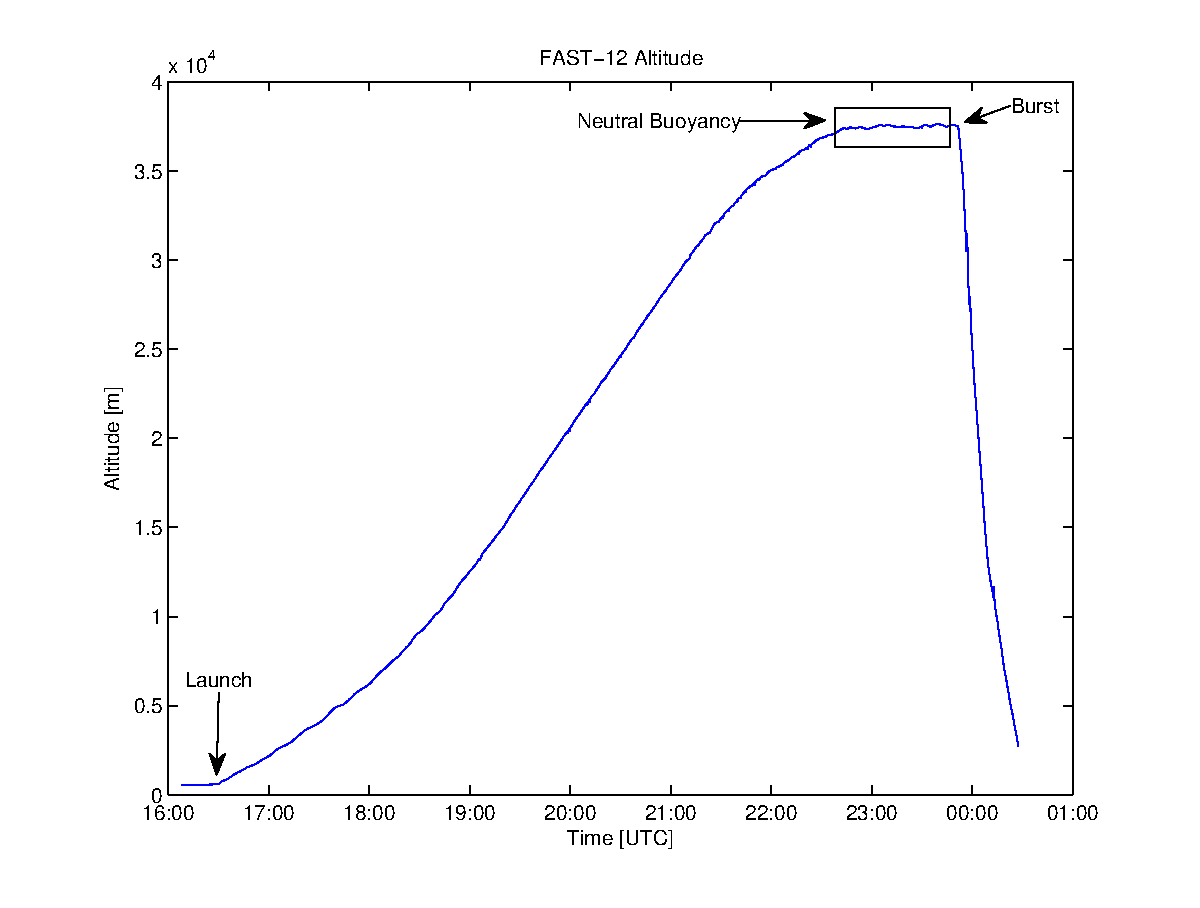
\includegraphics[width=0.5\textwidth]{altitude.eps}
  \caption{Altitude of neutrally-buoyant balloon vs. time}
\end{center}
\end{figure}



\label{lastpage}
\bibliography{sources}
\end{document}
